\newpage
\subsection{Press fit}
	\paragraph{Problem} A spur gear is mounted by press fit on a rotating shaft (figure \ref{ex:pressfit}). The nominal power of the transmission is $25kW$ with a service factor $K_s = 1.2$ and a rotational speed $n = 1000rpm$. Determine
	\begin{enumerate}[a)]
		\item the minimum and the maximum interference;
		\item the coupling tolerances;
		\item safety margin on the maximum transmittable torque;
		\item the stress state.
	\end{enumerate}
	Known datas are: $L = 40mm, D_c = 60mm, D_o = 400mm$, friction coefficient $f = 0.2$, safety against slipping $\phi = 1.25$ and against yielding $\phi_{ys} = 1.5$; for both shaft and gear consider $E = 210 GPa, \nu = 0.3, \sys = 450MPa$.
	
	\begin{SCfigure}[1.5][bh]
		\centering 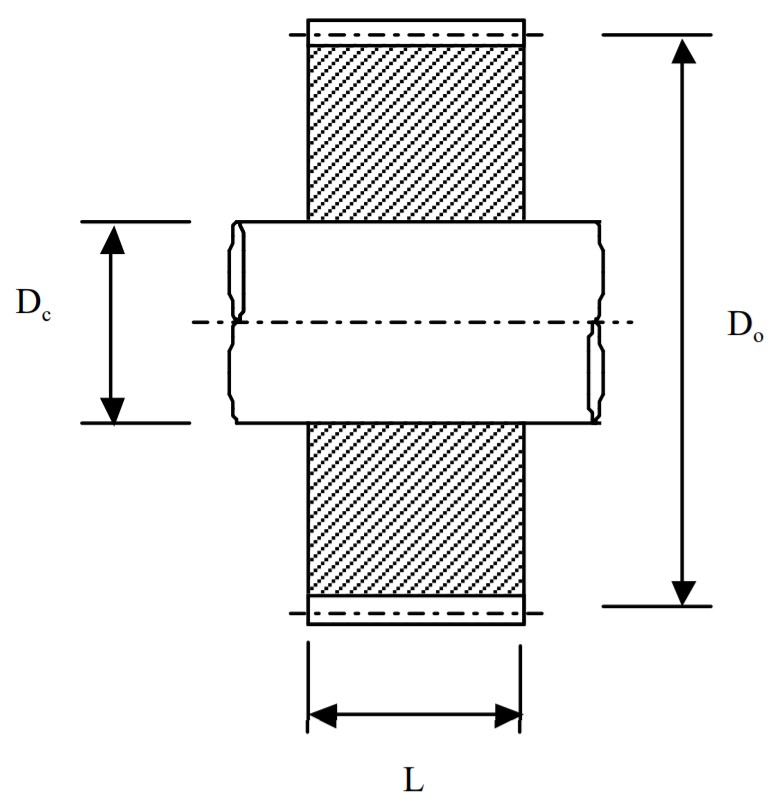
\includegraphics[width=6cm]{ex-pressfit} 
		\caption{sketch of a spur gear mounted by press fit on a rotating shaft.}
		\label{ex:pressfit}
	\end{SCfigure}

	\paragraph{Solution}
\begin{enumerate}[a)]
	
	\item The first thing to find the solution is determine the torque $T$ that has to be transmitted and so
	\[ T =  K_s \frac P \omega \qquad \xrightarrow{\omega = \frac{2\pi}{60} n} \quad T = K_s \frac{60}{2\pi} \frac{P}{n} = 286\, 479 N\cdot mm \]
	This means that the minimum contact pressure $p_{c,min}$ is related to the tangential stress $\tau$ produced by the torque $T$ at the interface, meaning
	\[ \tau = \frac{T}{r_c (2\pi r_cL)} = 1.267 MPa \]
	where $r_c \approx D_c/2$. With that stated the minimum contact pressure must be
	\[ p_{c,min} = \phi \frac \tau f = 7.916MPa \]
	where also the safety factor against slipping has been considered. By now using equation \ref{eq:interferencesimple} it's possible to compute the minimum interference as
	\[ i_{min} = 2 \frac{p_{c,min} r_c}{E} \frac 1 {1-\frac{r_c^2}{R_o^2}} = 0.00231 mm \]
	
	The maximum interference is instead dictated by the yielding condition, and so recalling equation \ref{eq:maxinterference}:
	\[2 |p_{c,max}| \frac 1 {1- \frac{r_c^2}{R_o^2}} \leq \frac{\sys}{\phi} \qquad \Rightarrow \qquad p_{c,max} = \frac{\sys}{2\phi_{ys}} \left( 1 - \frac{r_c^2}{R_o^2} \right) = 146.63 MPa \]
	Since the relation between interference and pressure is linear we can scale the minimum interference by the ration between maximum and minimum pressure, giving
	\[ i_{max} = \frac{p_{c,max}}{p_{c,min}} i_{min} = 0.0429 mm\]
	
	\item determining the diametral maximum and minimum interference as $\delta_{max} = 2i_{max} = 85.8\mu m$ and $\delta_{min} =  4.62\mu m$, we can look at table \ref{tab:metricfits} to check coupling feasibility. Considering the hole-base coupling \texttt{H6p5} we have that the tolerances (from the nominal diameter $D_c$) can be expressed as
	\[ \textrm{hub: } [0,19] \mu m \hspace{3cm} \textrm{hole: } [32, 32+13] = [32, 45]\mu m \]
	with such tolerances we have that the actual interferences lies inside the range of the theoretical values previously calculated:
	\[ 4.62 \mu mu < 32-19 \mu m = 13 \mu m < \delta < 45-0 \mu m = 45 \mu m < 85.8 \mu m \] 
	so the coupling \texttt{H6p5} fits for the problem.
	
	\item Considering the minimum interference of the chosen hole-base coupling as $i_{min} = 13/2 = 6.5 \mu m$, considering equation \ref{eq:interferencesimple} we have that the related minimum pressure is
	\[ p_{c,min,tol} = \frac{i_{min}E}{ 2 r_c} \left( 1 - \frac{r_c^2}{R_o^2}\right) = 22.24 MPa  \]
	then in the most critical condition we have
	\[ f p_{c,min,tol} = \frac{T_{tol}}{r_c (2\pi r_c L)} \qquad \Rightarrow \qquad T_{tol} = 2\pi fp_{c,min,tol}r_c^2 L = 1\,060\,000 N\cdot mm \]
	and so the safety margin on the transmissible torque is $\eta = T_{tol} / T = 3.51$.
	
	\item the stress state on the hub and the shaft can be computed using equation \ref{eq:pressstress}; with the properties of the problem we have that
	\[ \sigma_r = A - \frac B {r^2} \qquad \sigma_\theta = A + \frac B {r^2} \hspace{2cm} \textrm{with } \qquad A = \frac{p_c r_c^2}{R_o^2-r_c^2} \qquad B = \frac{p_c}{R_o^2-r_c^2} r_c^2R_o^2 \]
	Considering the maximum $p_{c,max,tol} = 77MPa $ and minimum $p_{c,min,tol} = 22.24MPa$ pressures for the tolerances related to the chosen hole-base coupling, we can then plot the stress state depending on such conditions (figure \ref{ex:pressstates}).
	\begin{SCfigure}[1][bht]
		\centering 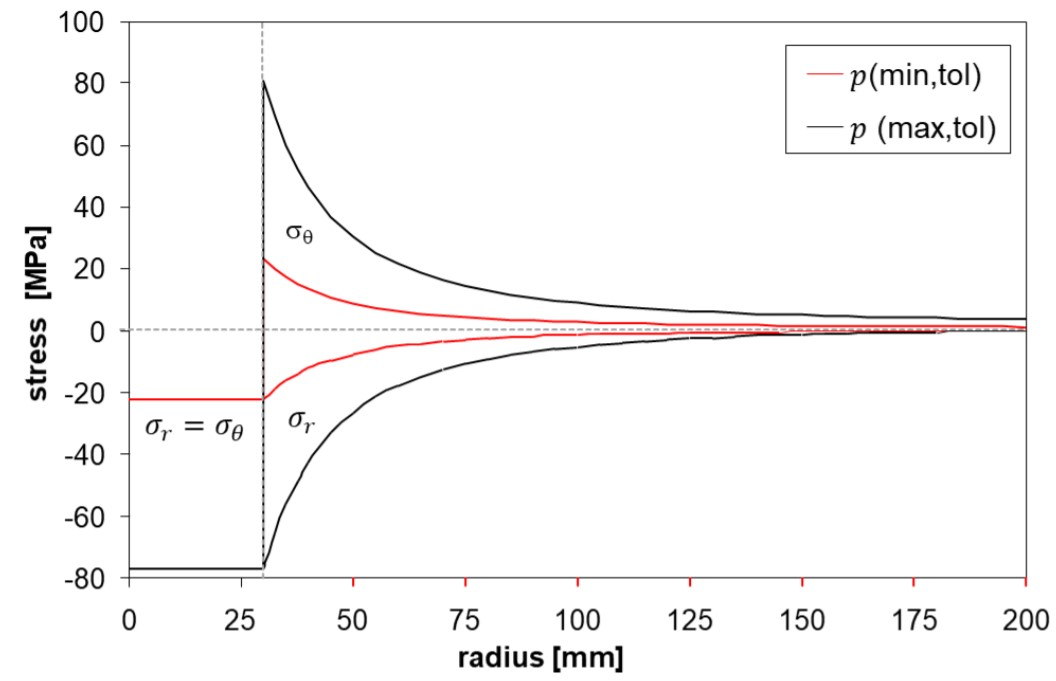
\includegraphics[width = 7cm]{pressfit-stresses}
		\caption{stress states in the shaft and the gear due to press fit connection in case of minimum and maximum tolerance coupling.} \label{ex:pressstates}
	\end{SCfigure}
	
	
	
	
	
	
	
	
	
	
	
	
	
	
\end{enumerate}